\begin{spacing}{1.3}
    \section{Lower Bound for Comparison Sorts}

    So far, all sorting algorithms we have seen perform no better than $\Omega (n \log n)$. 
    You may wonder if it is possible to have a much faster sorting algorithm,
    and the answer is No, if we {\it restricted to comparison sorts}, i.e., each time we 
    compare two numbers and decide some kind of order of them. All sorting algorithm we have seen 
    are {\bf comparison-based} sorts, and we can prove that any sorting algorithm based only on 
    comparison cannot perform better than $\Omega (n\log n)$.

    \begin{theorem}
        Any comparison sort algorithm requires $\Omega (n\log n)$ comparisons in the worst case.
    \end{theorem}

    Note that the correctness of the theorem above directly gives ``$\Omega(n\log n)$ is a 
    lower bound for all {\bf Comparison-Based Sorting} algorithms.''

    To proof the theorem, we first introduce {\bf Decision Tree}, with which we can view 
    the process of comparison sorts. 
    \begin{definition}
        A {\bf decision tree} is a {\it full binary tree} that represents the comparisons between 
        elements that are performed by a particular sorting algorithm on an input of given size.
    \end{definition}
    In a decision tree, each {\it non-leaf} node is represented by $i:j$ to indicate that we are comparing 
    $i$ and $j$, and if $i\le j$, we go to the left subtree, while $i>j$ goes to the right.
    Each {\it leaf} node represents a permutation of the result of sorting algorithm, corresponding to 
    an order of all items.

    The example below can help you have a better understanding of decision tree.
    \begin{center}
        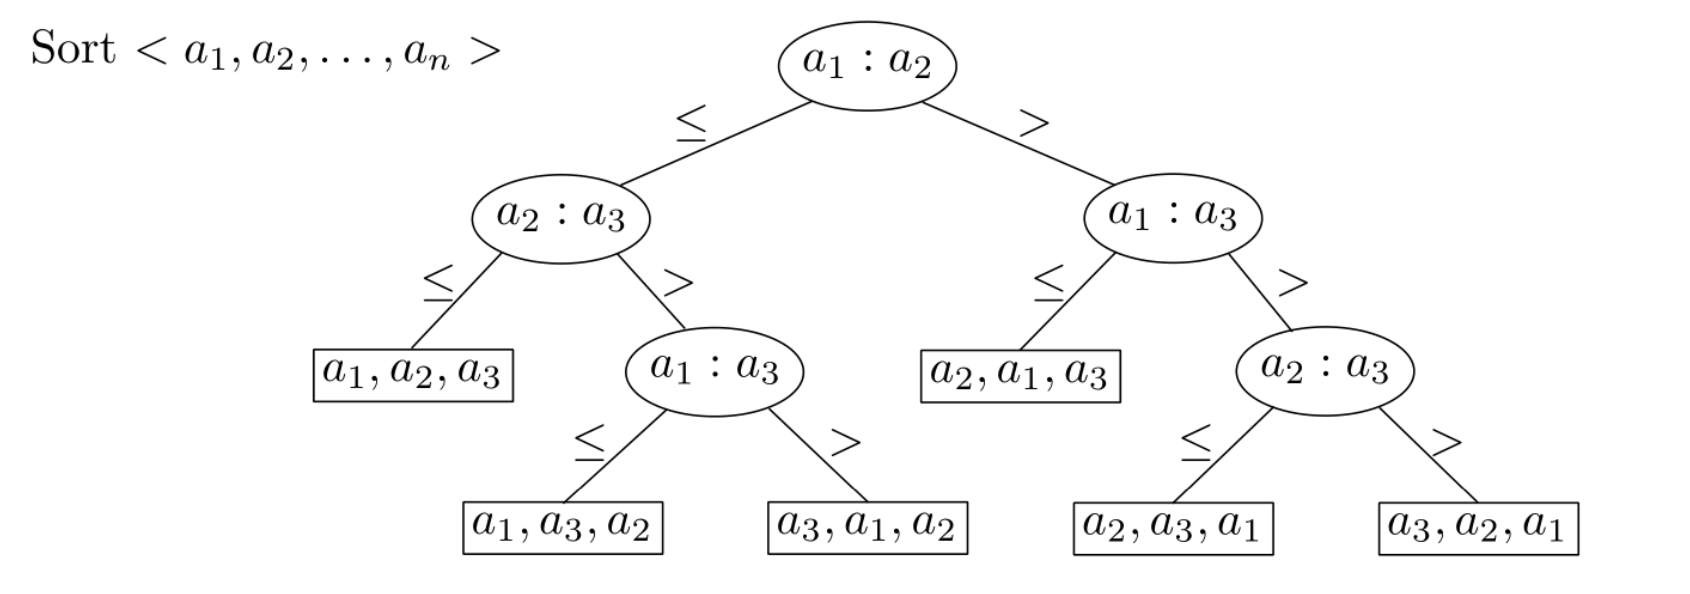
\includegraphics[scale=0.45]{images/06-decision-tree.png}
    \end{center}

    So the decision tree above basically imitates the process of our comparison sort,
    for example, we first ask ``Is $a_1$ larger than $a_2$?'', assuming the answer is 
    No, we go to left subtree, and then ask ``Is $a_2$ larger than $a_3$?'', and if 
    the answer is also No, we go to left subtree again, and reach a leaf node, 
    which means now we can determine their order, which is $a_1\le a_2\le a_3$.

    Notice that any correct sorting algorithm must be able to produce {\it each 
    permutation} of its input, each of the $n!$ permutations of a size $n$ input 
    must appear as one of the leaves of the decision tree for a comparison sort to be correct.
    (think why, though this is intuitive)

    Therefore, the decision tree must have $n!$ leaves since a sorting algorithm 
    can have $n!$ different outputs for each possible permutation on $n$ items.
    Moreover, a binary tree(recall decision tree is binary) with $n!$ leaves must 
    have height $\Omega(\log n)$(see theorem below). Therefore, the height of 
    tree must be 
    $$\Omega (\log (n!))=\Omega(n\log n)$$
    which means we need $\Omega(n\log n)$ comparisons in this algorithm, 
    therefore comparison-based sorting algorithm requires at least $\Omega(n\log n)$ time.

    \begin{theorem}
        A binary tree with $n$ leaves must have height $\Omega (\log n)$.
        \begin{proof}
            Firstly we know a binary tree of height $h$ has at most $2^h$ leaves.
            (This should follow immediately from the definition of binary tree)
            Since the tree has $n$ leaves, we have 
            $$n\le 2^h\quad \Rightarrow h\ge \log_2 n$$
        \end{proof}
    \end{theorem}


    
    \newpage
    \section{Counting Sort}
    So, it is true that we cannot do better for sorting? No! 
    We may consider other sort algorithms that doesn't depend on comparisons.

    Here is one intuitive method. Consider you have $n$ integers and all of them 
    are between $1$ and $k$. For example, if $n=5$ and $k=4$, you may have:
    $$a_1=4\quad a_2=2\quad a_3=1\quad a_4=4\quad a_5=2$$
    Now consider you have $k$ ``buckets'', labelled from $1$ to $k$, whenever you meet 
    an item $x$, you put it into the bucket with label $x$. Now your buckets should look like:
    \begin{center}
        \begin{tabular}{r|C{2cm}|C{2cm}|C{2cm}|C{2cm}}
            \hline
            Bucket & 1 & 2 & 3 & 4\\\hline
            \# of items in the bucket & 1 & 2 & 0 & 2\\\hline
        \end{tabular}
    \end{center}
    because you have one 1, two 2s and two 4s.

    Now if you have those ``buckets'', it will be easy for you to sort those numbers,
    for example, $a_5$ should be put at new position 3, since there are 
    one item in bucket 1, and two items in bucket 2(one of the two items is $a_5$ itself)
    that are less than or equal to $a_5$. So the new order will be:
    \begin{center}
        \begin{tabular}{r|C{2cm}|C{2cm}|C{2cm}|C{2cm}|C{2cm}}
            \hline
            Order after sorting & 1 & 2 & 3 & 4 & 5\\\hline
            Item &  &  & $a_5=2$ & & \\\hline
        \end{tabular}
    \end{center}
    Notice if we first check $a_2$, then it will also be put at new position 3, 
    for the same reason above. However, we would not do that because it will 
    lead to {\it unstable sort}. Notice that $a_2=a_5=2$ at the beginning, 
    so if the sort is {\it stable}, we still want $a_2$ to be in front of $a_5$ 
    after sorting. Inspired by this, we should {\it check items backwards},
    i.e., check $a_5$, then $a_4$, then $a_3$, $a_2$, $a_1$. This guarantee
    our algorithm to be {\it stable}. (please think about this point twice,
    it is important for you to know why check backwards can make it stable)

    Back to our sorting process, remember we check items {\it backwards}, 
    so now we check $a_4$. Similarly, $a_4$
    should be put at new position 5, since there are 
    one item in bucket 1, two items in bucket 2 and two items in 
    bucket 4(one of the two items is $a_4$ itself)
    that are less than or equal to $a_4$.
    \begin{center}
        \begin{tabular}{r|C{2cm}|C{2cm}|C{2cm}|C{2cm}|C{2cm}}
            \hline
            Order after sorting & 1 & 2 & 3 & 4 & 5\\\hline
            Item &  &  & $a_5=2$ & & $a_4=4$\\\hline
        \end{tabular}
    \end{center}
    Then $a_3$, there is only one item in bucket 1, which is $a_3$ itself, 
    so it should be put at position 1.
    \begin{center}
        \begin{tabular}{r|C{2cm}|C{2cm}|C{2cm}|C{2cm}|C{2cm}}
            \hline
            Order after sorting & 1 & 2 & 3 & 4 & 5\\\hline
            Item & $a_3=1$ &  & $a_5=2$ & & $a_4=4$\\\hline
        \end{tabular}
    \end{center}
    Then $a_2$, notice though there are 
    one item in bucket 1, and two items in bucket 2(one of the two items is $a_2$ itself)
    that are less than or equal to $a_2$, we have {\it already ejected $a_5$},
    so now it should be put at position $1+1=2$ rather than $1+2=3$.
    (think twice, make sure you understand the process)
    \begin{center}
        \begin{tabular}{r|C{2cm}|C{2cm}|C{2cm}|C{2cm}|C{2cm}}
            \hline
            Order after sorting & 1 & 2 & 3 & 4 & 5\\\hline
            Item & $a_3=1$ & $a_2=2$ & $a_5=2$ & & $a_4=4$\\\hline
        \end{tabular}
    \end{center}
    Then $a_1$, similar to $a_2$, it should be put at position $1+2+1=4$ rather than 
    $1+2+2=5$ since $a_4$, which equals to $a_1$, has already been ejected.
    \begin{center}
        \begin{tabular}{r|C{2cm}|C{2cm}|C{2cm}|C{2cm}|C{2cm}}
            \hline
            Order after sorting & 1 & 2 & 3 & 4 & 5\\\hline
            Item & $a_3=1$ & $a_2=2$ & $a_5=2$ & $a_1=4$ & $a_4=4$\\\hline
        \end{tabular}
    \end{center}
    Now the sorting process terminates, with order $a_3, a_2, a_5, a_1, a_4$, 
    with no surprise, this is a {\it stable sort algorithm}.

    \begin{remark}
        {\bf Remark:} After the whole process, try to recall:
        \begin{itemize}
            \item What do the ``buckets'' hold?
            \item Why we check items backwards?
            \item How do we determine the position of an item?
            \item Why sometimes we need to ``kick-out'' some elements, rather 
            than simply add up the number of items in all buckets that are less than 
            or equal to it?
        \end{itemize}
    \end{remark}

    The code of this algorithm could be rather confusing. 
    In code, after computing how many items should each ``bucket'' holds, we 
    replace them with how many items that are {\it less than or equal to} the 
    ``bucket label'', that is, a {\it prefix sum} of the ``buckets''.
    If you redo the process above, you can discover that this will largely 
    reduce the complexity of the process: when we determine the position of 
    element $x$, we don't need to calculate how many items are less than or equal to $x$,
    we can directly read off from ``bucket'', also, when position of $x$ is determined,
    we decrease the number stored in ``bucket'' $x$ by 1, indicating {\it we have 
    already ejected one $x$ out, and we should not re-count it when we meet another 
    $x$ later}.
    
    \newpage
    \begin{algorithm*}
        \setstretch{1.1}
        \caption{Counting-Sort($A$, $B$, $n$, $k$)}
        \KwIn{$A[1\cdots n]$, where $A[i]\in \{1,2,\cdots, k\}$}
        \KwOut{$B[1\cdots n]$, sorted $A$ array}
        \tcp{$C[i]$ will be our ``bucket'' with label $i$}

        Let $C[1\cdots k]$ be a new array with all 0

        \For{$i\lar 1$ to $n$}{
            \tcp{For item $A[i]$, put it into ``bucket'' with label $A[i]$}

            $C[A[i]]\lar C[A[i]] + 1$
        }

        \For{$j\lar 2$ to $k$}{
            $C[j]\lar C[j] + C[j-1]$\qquad \tcp{prefix-sum, as we explained before}
        }
        \tcp{Now $C[i]$ stores the number of items that $\le i$}

        \tcp{Now check backwards, determine the position of each item}
        \For{$j\lar n$ to $1$}{
            \tcp{item $A[j]$ has $C[A[j]]$ items $\le $ it, 
            so it should at position $C[A[j]]$}

            $B[C[A[j]]]\lar A[j]$ \\

            \tcp{
                Remember we have ejected one $A[j]$, should not re-count when meet another $A[j]$ later
            }

            $C[A[j]]\lar C[A[j]] - 1$
        }
    \end{algorithm*}
    Running time: $\Theta(n+k)$.

    This process is only slightly different from what we introduced above.
    I'd like to attach a picture in textbook for your reference, which 
    shows the detail steps of what the algorithm given above is doing.
    \begin{center}
        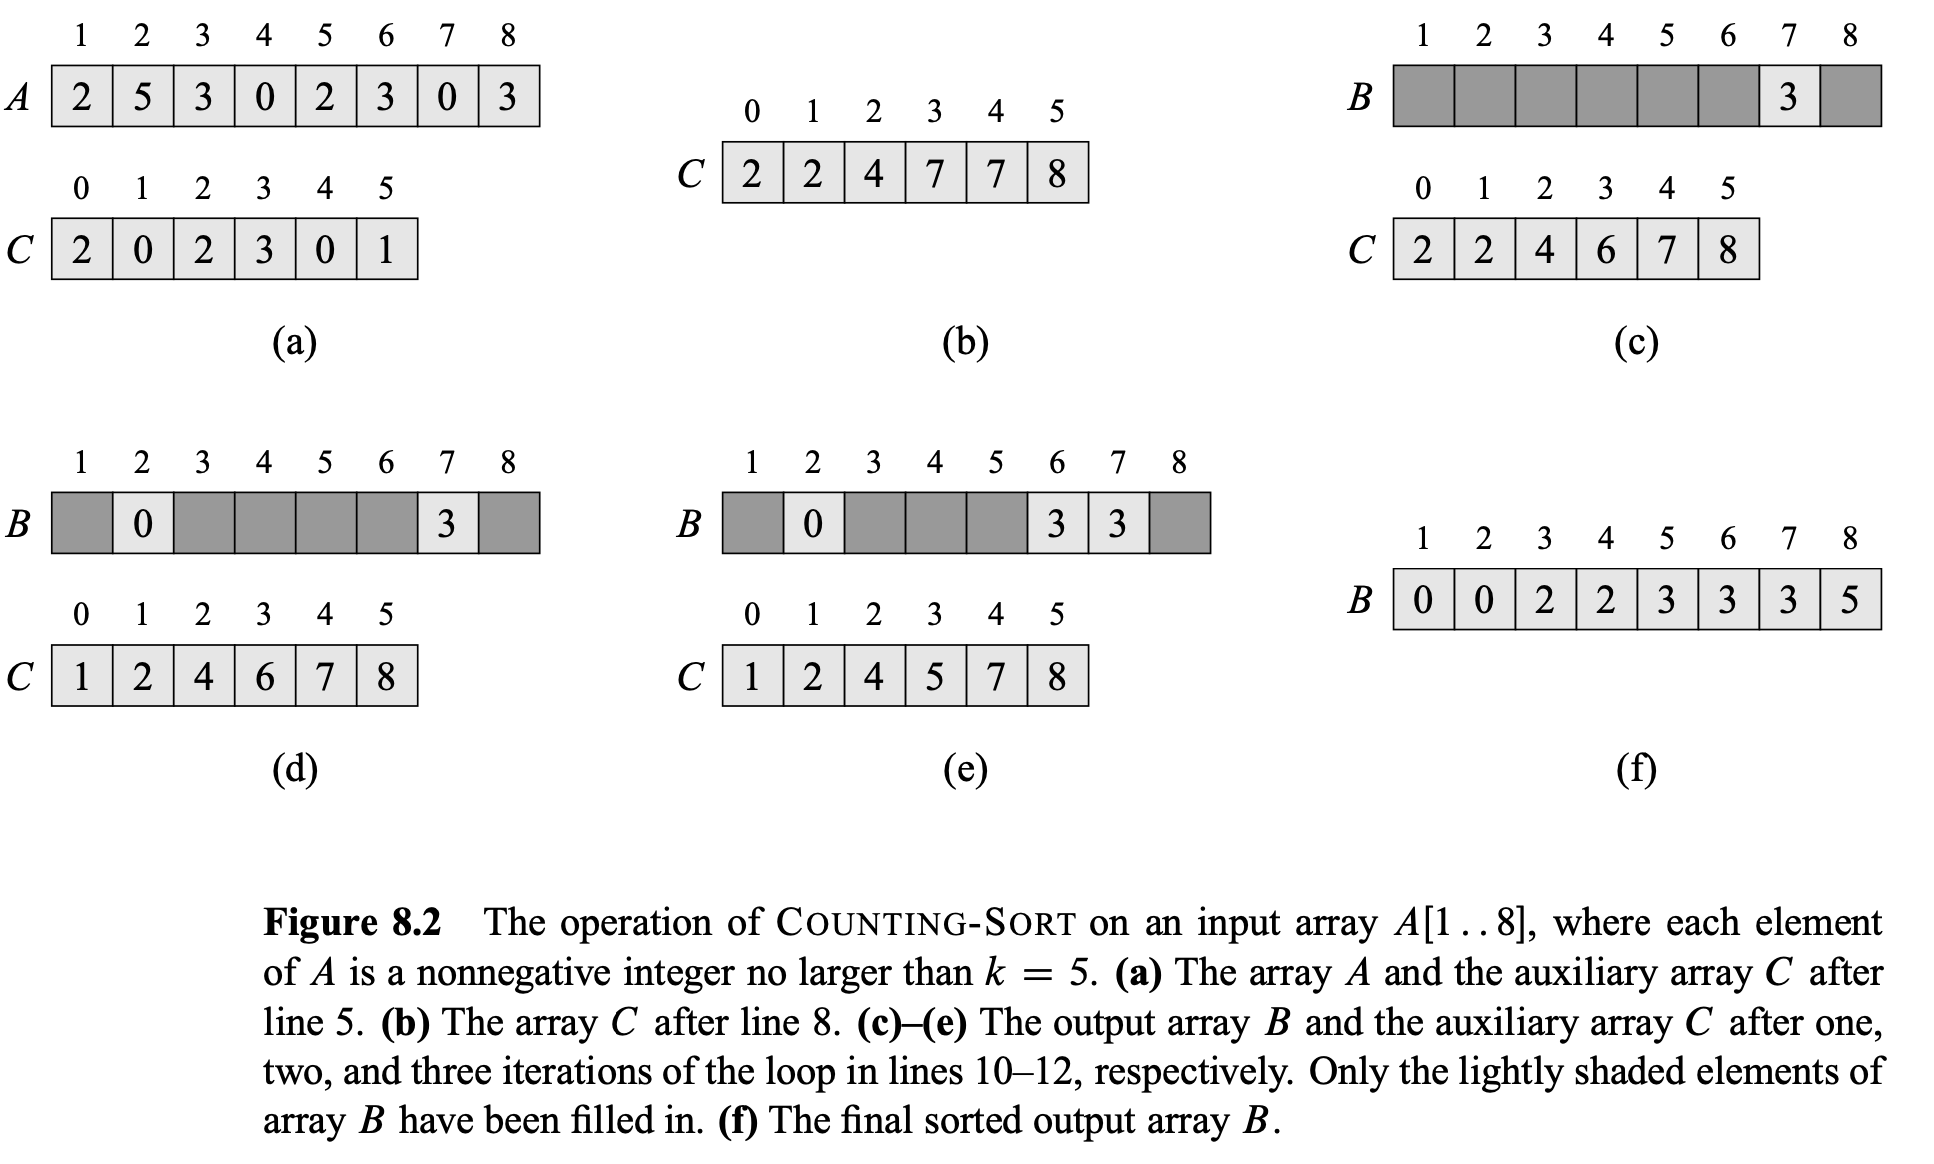
\includegraphics[scale=0.43]{images/06-counting-eg.png}
    \end{center}
    

    \section{Radix Sort}

    {\bf Radix Sort} is quite interesting. With the help of a {\it stable 
    sort}, where Counting Sort will be a good choice, it sorts the array 
    on one digit, each time, from {\bf least-significant bit}(LSB) to 
    {\bf most-significant bit}(MSB).

    Here is what Radix Sort does, on an input of array of $n$ items,
    each of them has $d$ digits, and digit $1$ is the right-most digit(LSB),
    digit $d$ is the left-most digit(MSB).

    \begin{algorithm*}
        \caption{Radix-Sort($A,d$)}
        \For{$i\lar 1$ to $d$}{
            use {\bf counting sort} to sort array $A$ on digit $i$
        }
    \end{algorithm*}
    Here is an example of what Radix Sort does on each step:
    \begin{center}
        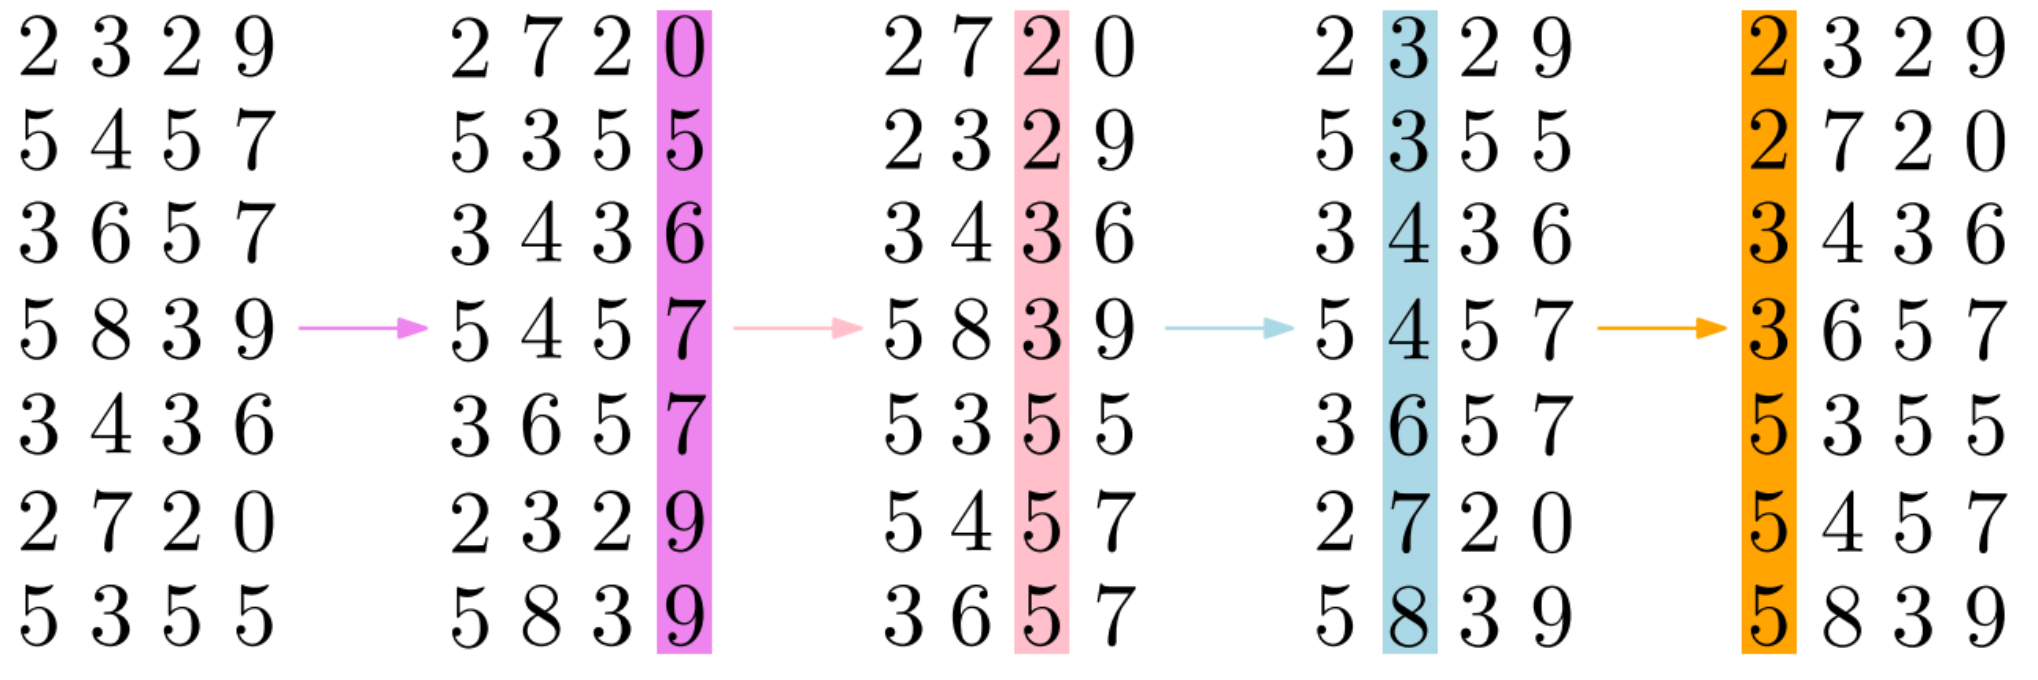
\includegraphics[scale=0.4]{images/06-radix-eg.png}
    \end{center}
    Since here we are focusing on decimal numbers, so for counting sort, 
    $k=10$(each digit is in $\{0,1,\cdots, k-1\}$). It is not necessary that 
    we sort it on decimal numbers, actually each digit can be of any range,
    maybe hexadecimal, binary, etc, since all of them work fine with 
    Counting Sort.

    We prove the correctness of Radix Sort by induction.
    \begin{proof}
        Assume that the numbers are already sorted by their low-order $i-1$ digits.
        (that is, we've already use radix sort on digit $1\cdots i-1$)

        Now assume sorting on digit $i$. 
        \begin{itemize}
            \item Two numbers that differ on digit $i$ will be correctly sorted 
            by their $i-$th digit, 
            \item Two numbers that we same digit $i$ will be put in the same order 
            in output as they were in input, since we are using a stable sort,
            (Counting Sort, usually)
        \end{itemize}
        Therefore, they are correctly sorted by their $i-$th digits.
    \end{proof}

    The running time of Radix Sort is depends on three variables: $n$, the size of input, 
    $k$, the numbers of values that each digit can take, and $d$, number of digits 
    in each item.

    We know Counting Sort takes $\Theta(n+k)$ time, and for Radix Sort, we run 
    Counting Sort for $d$ times, its running time should be $\Theta(d(n+k))$.

    If you remember what we said above, it is not necessary that we represent each 
    item in decimal numbers. If we are given $n$ hexadecimal numbers, $k$ changes 
    from $10$ to $16$, but $d$ will become smaller. On the contrary, if we are given 
    $n$ binary numbers, $k$ will be only 2, but $d$ will become larger.


    \section{Sort Review}

    For now, you've seen those sorting algorithms.
    \begin{center}
        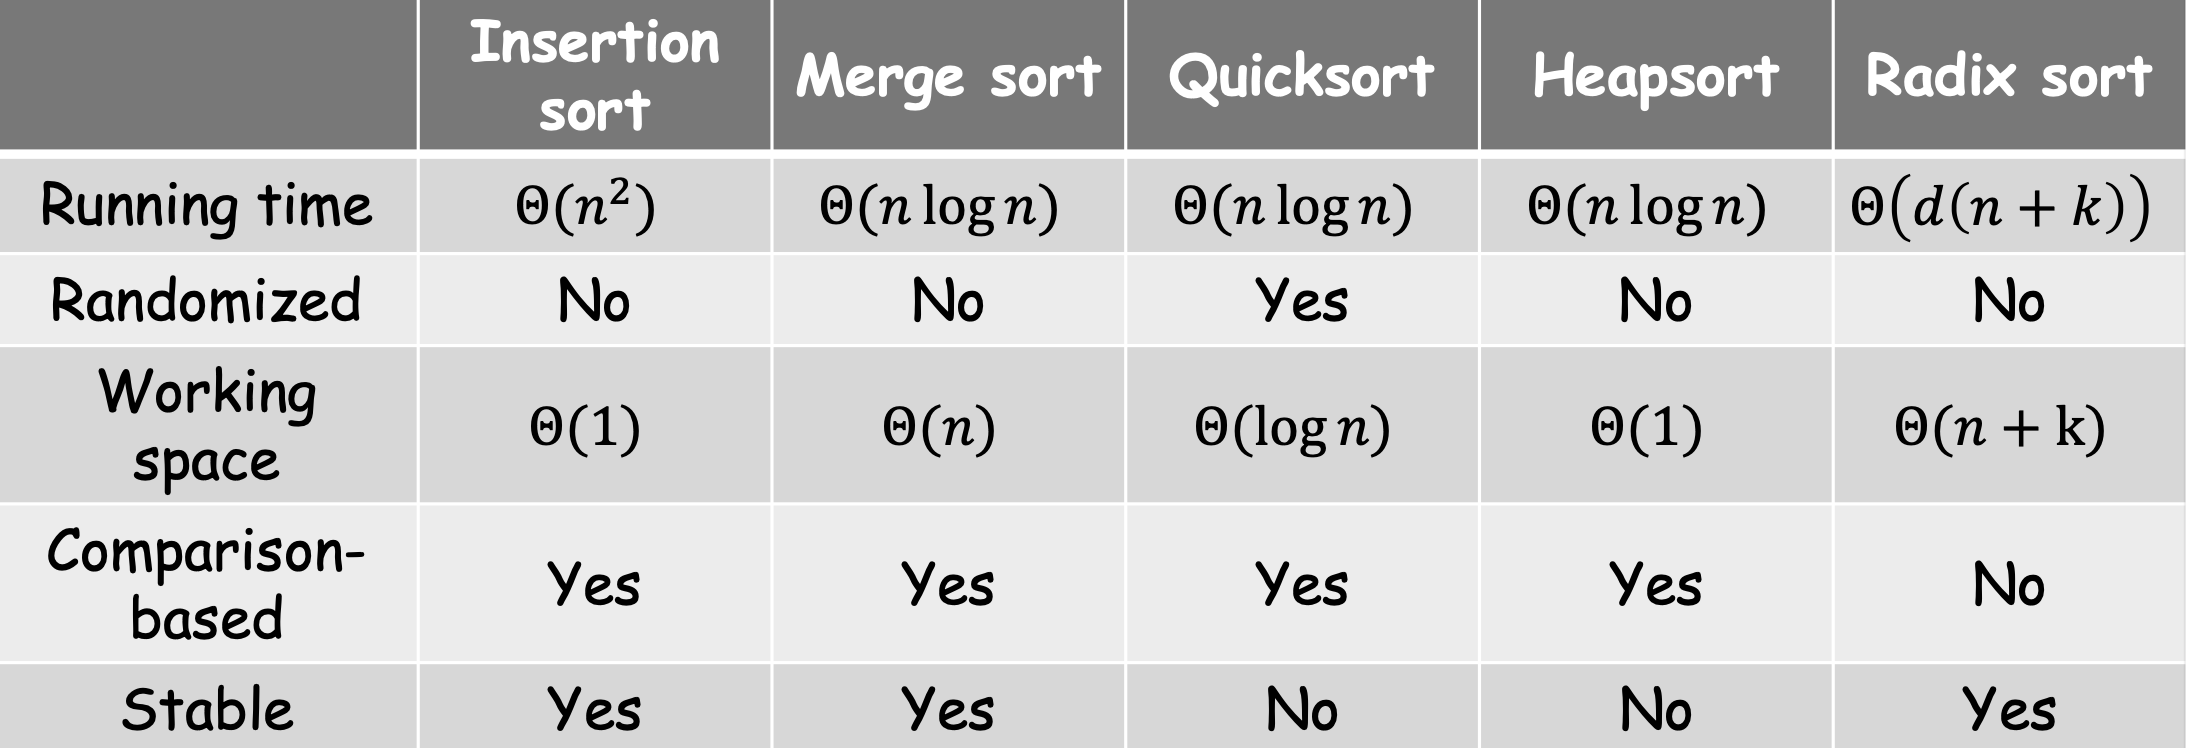
\includegraphics[scale=0.4]{images/06-sort-review.png}
    \end{center}

    
\end{spacing}